%\chapter{The Optimum Receiver}

%\subsection{Problem}
%
\begin{problem}
Type the following program in octave to obtain $g(t)$.  $g(t)$ is a periodic signal called a square wave with amplitude $A = 5V$ and time period $T=20 ms$.
\end{problem}
%
\solution
\lstinputlisting[language=octave]{./chapter1/codes/1.1.m}
\begin{figure}[!h]
\centering

%\includegraphics[width=0.7\linewidth]{chapter1/clock}
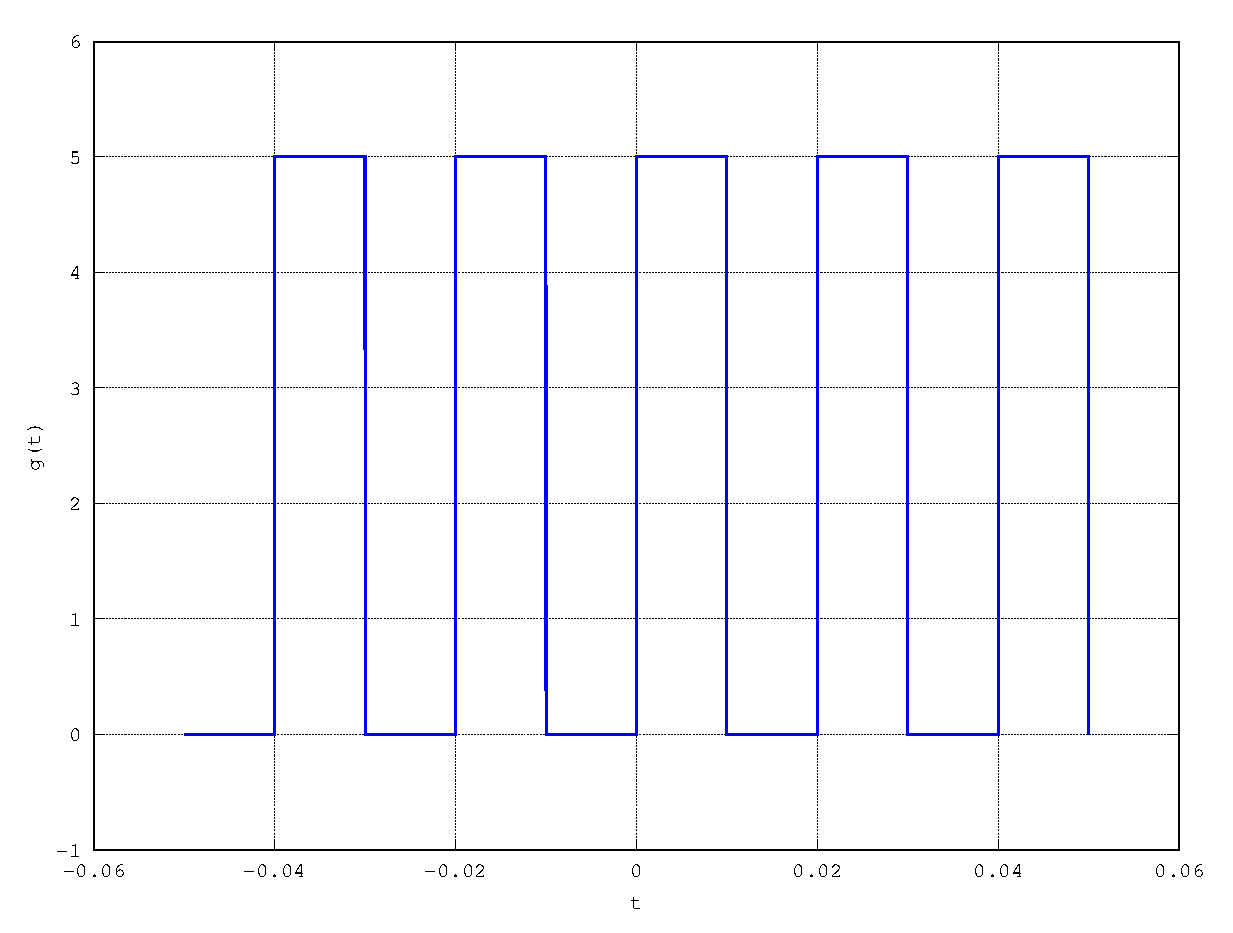
\includegraphics[width=\columnwidth]{./chapter1/figs/1.1.eps}
%\vspace*{-13cm}
\caption{Generating square wave.}
\label{fig:1.1}
\end{figure}
\begin{problem}
The following expression
%
\begin{equation}
g(t) = \sum_{n=0}^{\infty}a_n\cos 2\pi n f t + b_n \sin 2 \pi n f t
\end{equation}
is known as the Fourier series expansion of $g(t)$, where $f = \frac{1}{T}$.  Find 
\begin{align}
a_n &= \frac{2}{T} \int_{0}^{T}g(t) \cos 2\pi nf t \, dt \\
b_n &= \frac{2}{T} \int_{0}^{T}g(t) \sin 2\pi nf t \, dt
\end{align}
\end{problem}
%
\solution 
\begin{align}
a_0 &= \frac{A}{T} \int_{0}^{T_0}  dt \\
&= \frac{AT_0}{T}
\end{align}
and
\begin{align}
a_n &= \frac{2A}{T} \int_{0}^{T_0}\cos 2\pi nf t \,  dt \\
&= \frac{A}{\pi n f T }\sin 2\pi n f T_0
\end{align}
Similarly, 
\begin{align}
b_n &= \frac{2A}{T} \int_{0}^{T_0}\sin 2\pi nf t \,  dt \\
&= \frac{A}{\pi n f T }\sbrak{1 - \cos 2\pi n f T_0}
\end{align}

%
\begin{problem}
Using Octave, compute the series 
%
\begin{equation}
\sum_{n=0}^{15}a_n\cos 2\pi n f t + b_n \sin 2 \pi n f t
\end{equation}
%
for $A=5, T= 20 ms$ and $a_n,b_n$ obtained in the previous problem.  Comment.
%
\label{fourier_series}
\end{problem}
\solution  Type the following program
%
\lstinputlisting[language=octave]{./chapter1/codes/1.4.m}
to obtain the following figure.
\begin{figure}[!h]
\centering

%\includegraphics[width=0.7\linewidth]{chapter1/clock}
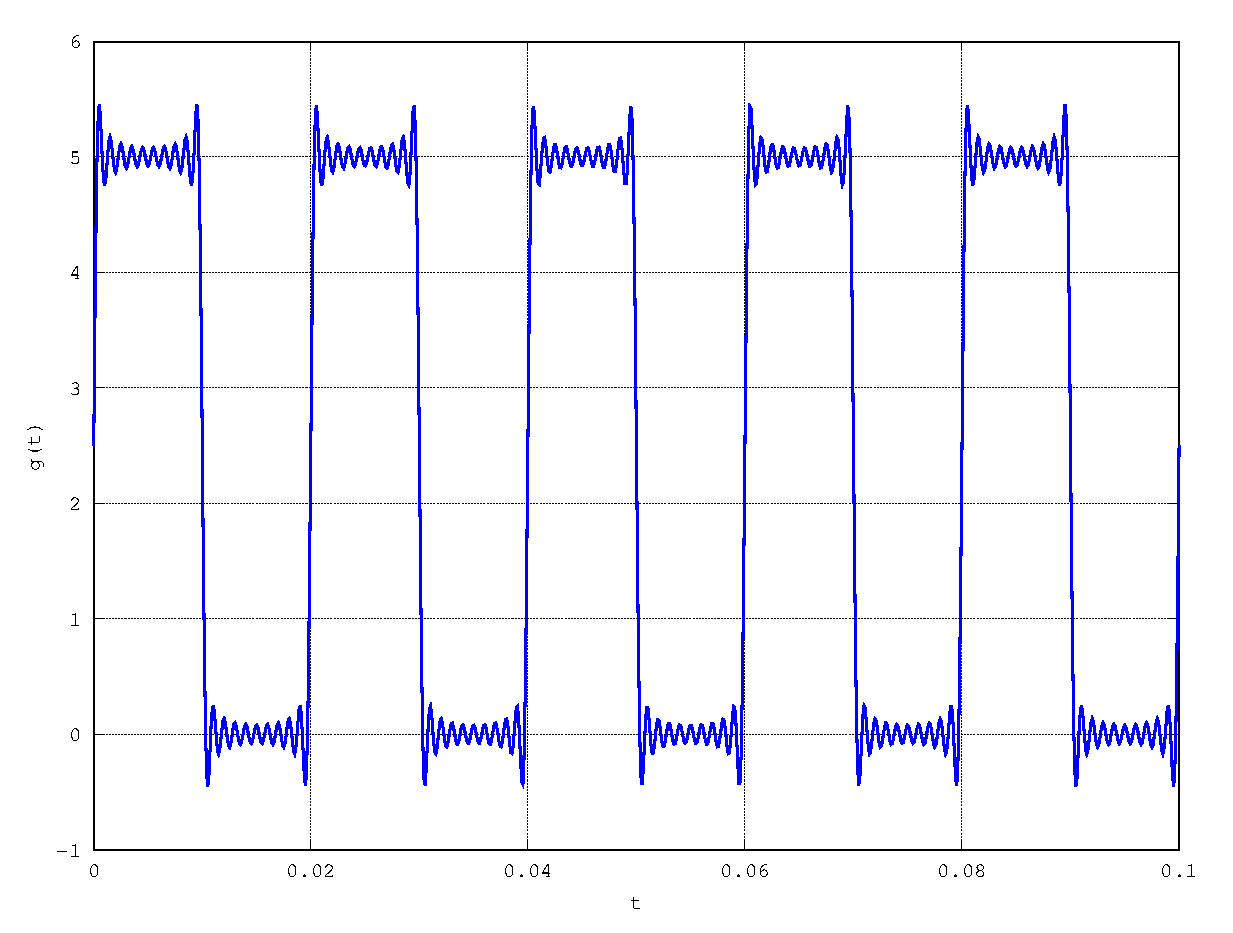
\includegraphics[width=\columnwidth]{./chapter1/figs/1.4.eps}
%\vspace*{-13cm}
\caption{Gibbs phenomenon.}
\label{fig:1.4}
\end{figure}
%
\begin{problem}
  Generate $g(t)$ using an arduino for $A = 5\, V$ and $T = 20 \, ms$ using the blink.ino program.
  \end{problem}
%

	%\begin{figure}[!h]
%\centering

%%\includegraphics[width=0.7\linewidth]{chapter1/clock}
%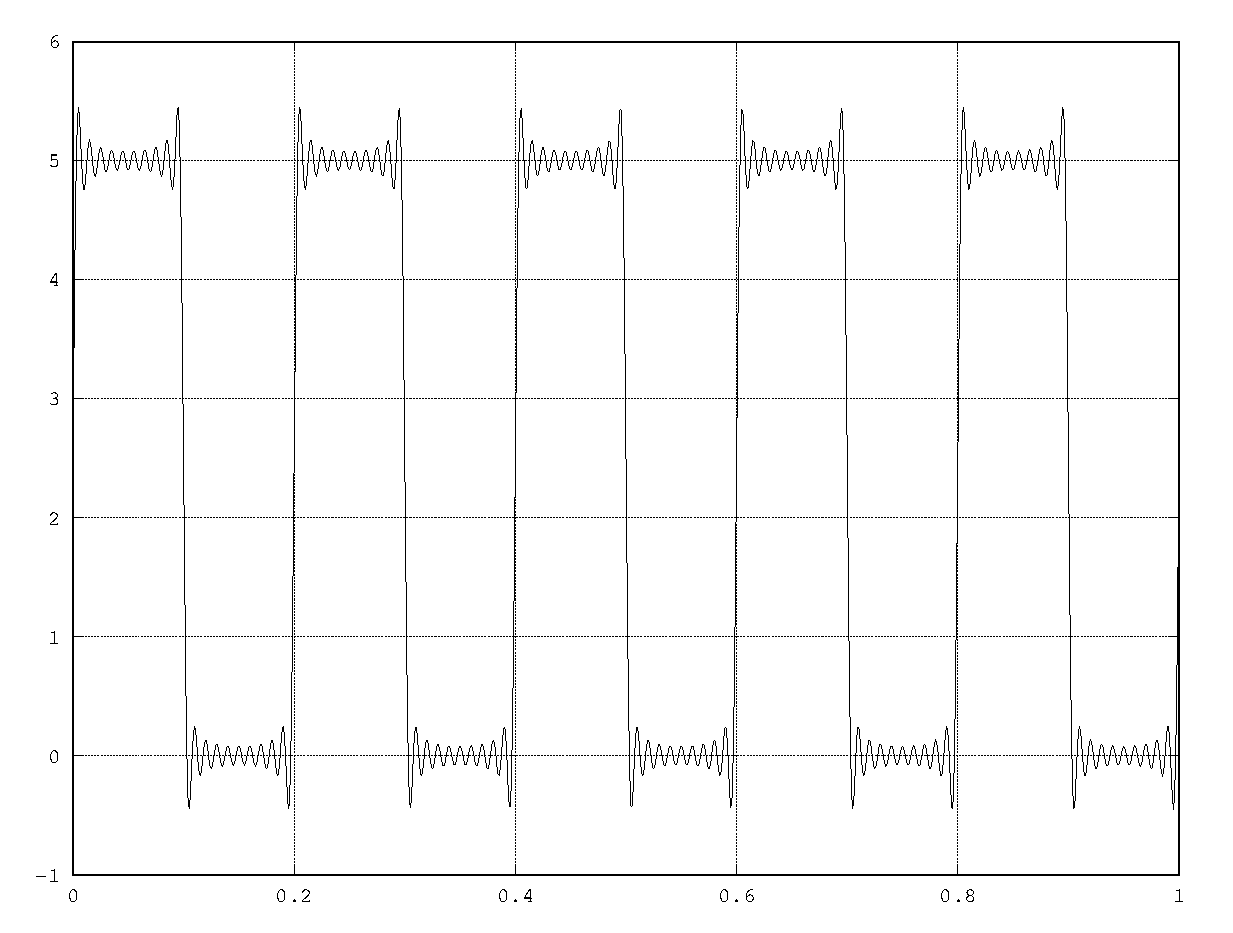
\includegraphics[width=\columnwidth]{chapter1/filter_input}
%%\vspace*{-13cm}
%\caption{Generating square wave using a fourier series.}
%\label{fig:clock}
%\end{figure}

